%% Progetto di linguaggi di programmazione - Gianluca Grilletti e Giovanni Barbarino
%% Semantica Fully Abstract per PCF


\documentclass{beamer}

\usepackage[utf8]{inputenc}
\usepackage{default}
\usepackage{amssymb}
\usepackage{stmaryrd}
\usepackage{graphicx}
\usepackage{caption}
\usepackage{xcolor}
%\usepackage{subcaption}
\usepackage{tikz}
\usetikzlibrary{arrows,automata}

\newcommand{\eqobs}{\stackrel{\text{obs}}{=}}
\newcommand{\limp}{\mathbin{{-}\mkern-3.5mu{\circ}}}


%%%% comandi tikz
\newcommand{\tnode}[4]{\node (#1_u) at (#2,#3+0.1) [minimum size=2pt, opacity=0]{#4};
		       \node (#1_d) at (#2,#3-0.1) [minimum size=2pt, opacity=0] {#4};
		       \node (#1) at (#2,#3) [minimum size=2pt] {#4};}



% immagini
\graphicspath{{immagini/}}




\usetheme{Darmstadt}
\setbeamercovered{dynamic}

\title{Un modello fully abstract del PCF}
% \subtitle{Vuoi fare un gioco con me?}
\author{Grilletti Gianluca \and Barbarino Giovanni}
\institute[Unipi]{Università di Pisa}


\begin{document}

\small


%titolo
\begin{frame}
	%\frametitle{Il linguaggio PCF}
	\maketitle
	
\end{frame}

\section{La categoria dei giochi}


\subsection{giochi e strategie}

% i giochi
\begin{frame}
	\frametitle{I giochi}
	
	Il modello che andremo a considerare si basa sulla \emph{teoria dei giochi}.
	
	
	Un \textbf{gioco} è una 4-upla $A=( M_A , \lambda_A , P_A , \approx_A )$ dove:
	\begin{itemize}
	\item<2-> $M_A$ è l'insieme delle mosse
	\item<3-> $\lambda_A$ è una funzione da $M_A$ all'insieme $\{ O,P\} \times \{Q,A\}$; in particolare:
		\begin{itemize}
		\item $O$ indica il giocatore "opponent" e $P$ il giocatore "player"
		\item $Q$ indica una domanda e $A$ una risposta
		\end{itemize}
	\item<4-> Una \textit{partita} è una stringa finita di mosse tale che:
		\begin{enumerate}
		\item La prima mossa è di $O$
		\item $P$ e $O$ si alternano
		\item In ogni sottostringa iniziale, il numero di risposte deve essere al più uguale al numero di domande (\emph{bracketing condition})
		\end{enumerate}
	\item<5-> $P_A$ è un sottoinsieme prefix-closed di partite; chiameremo $P_A$ l'insieme delle \textit{partite valide}
	\item<6->  $\approx_A$ è una relazione di equivalenza sulle partite valide
	\end{itemize}
	
	
\end{frame}

% tavolo e carte
\begin{frame}

\frametitle{Tavolo di Gioco}
	
	Possiamo rappresentare partite accettabili tramite il \emph{Tavolo di Gioco}
	
	\begin{columns}
	\begin{column}{0.45\textwidth}
	\only<2->{Gioco $A=( M_A , \lambda_A , P_A , \approx_A )$
		\begin{itemize}
		         	\item $M_{A}=\{*_1,*_2,n_1,n_2\}$
		           	\item $\lambda_{A}= \{ (*_1,OQ) ;$ $ (*_2,PQ) ; (n_1,PA) ; (n_2,OA) \}$
					\item $P_{A}= \{ 
					\only<3>{\textcolor{red}}{\epsilon} ,$
					$ \only<4>{\textcolor{red}}{*_1} ,
					\; *_1n_1, $ 
					$ \only<5>{\textcolor{red}}{*_1*_2},
					\; \only<6>{\textcolor{red}}{*_1*_2n_2}, 
					\; \only<7->{\textcolor{red}}{*_1*_2n_2n_1} \}$
					\item $\approx_{A} = id_{A}$        
		\end{itemize}}
	\end{column}
	\begin{column}{0.4\textwidth}
		\begin{tikzpicture}
			 \node (inv) at (0,0) [minimum size=2pt] {};
			 \node (inv2) at (4,-5) [minimum size=2pt, scale=1.5] {};
			 
	\only<3->{	 \draw [fill=blue, opacity=.5] (3.5,-4) rectangle (.5,-1);
			 \node (A) at (2,-2.5) [minimum size=2pt, scale=4] {A};
			 \node (P) at (1,-3.5) [minimum size=2pt, scale=2.5] {P};
			 \node (O) at (1,-1.5) [minimum size=2pt, scale=2.5] {O};}
			 
			 
			 
			 \only<4-> {\node (st_1) at (2.5,-.5) [minimum size=2pt, scale=1.5] {$*_1$};}
			 \only<5-> {\node (st_2) at (2.5,-4.5) [minimum size=2pt, scale=1.5] {$*_2$};}
			 \only<6->{\node (ri_1) at (1.5,-.5) [minimum size=2pt, scale=1.5] {$n_2$};}
			 \only<7->{\node (ri_2) at (1.5,-4.5) [minimum size=2pt, scale=1.5] {$n_1$};}
			 
			  \only<5->{\draw[->] [out=280,in=80] (st_1) to (st_2);}
			  \only<6->{\draw[->] [out=110,in=300] (st_2) to (ri_1);}
			  \only<7->{\draw[->] [out=280,in=80] (ri_1) to (ri_2);}
			  
			\end{tikzpicture}
		
	\end{column}
	\end{columns}

	\onslide<8-9> {
	
	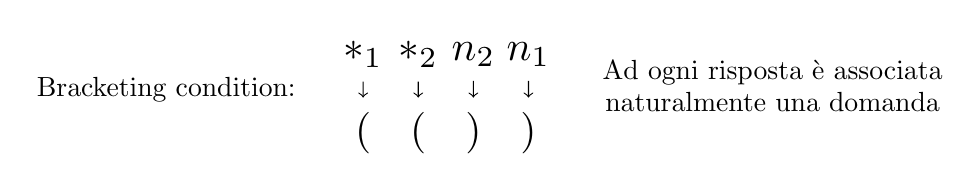
\begin{tikzpicture}
			
			\node (text) at (0,-.45) [minimum size=2pt] {Bracketing condition:};
			\only<9>{
			\node (text2) at (7.7,-.23) [minimum size=2pt] {Ad ogni risposta è associata};
			\node (text3) at (7.7,-.6) [minimum size=2pt] {naturalmente una domanda};
			}
			 \node (st1) at (2.5,0) [minimum size=2pt, scale=1.5] {$*_1$};
			 \node (st2) at (3.2,0) [minimum size=2pt, scale=1.5] {$*_2$};
			 \node (n2) at (3.9,0) [minimum size=2pt, scale=1.5] {$n_2$};
			 \node (n1) at (4.6,0) [minimum size=2pt, scale=1.5] {$n_1$};
			 
			 \node (pst1) at (2.5,-1) [minimum size=2pt, scale=1.5] {$($};
			 \node (pst2) at (3.2,-1) [minimum size=2pt, scale=1.5] {$($};
			 \node (pn2) at (3.9,-1) [minimum size=2pt, scale=1.5] {$)$};
			 \node (pn1) at (4.6,-1) [minimum size=2pt, scale=1.5] {$)$};
			 
			 \draw[->] (st1) to (pst1);
			 \draw[->] (st2) to (pst2);
			 \draw[->] (n1) to (pn1);
			 \draw[->] (n2) to (pn2);
				
			
			 
			  
	\end{tikzpicture}
	
	
	}
	
\end{frame}

% strategie
\begin{frame}

	\frametitle{Strategie}
	
	Una \textbf{strategia} $\sigma$ è un insieme di partite di lunghezza pari (l'ultima mossa è di $P$) tali che:
	\begin{itemize}
		\item<2-> $\sigma$ sia prefix-closed sulle partite di lunghezza pari
		\item<3-> $\sigma$ sia \textit{history free}, cioè
		\begin{itemize}
			\item $sab , tac \in \sigma \Rightarrow b=c$
			\item $sab, t\in \sigma, ta\in P_A \Rightarrow tab\in \sigma$
		\end{itemize}
	\end{itemize}
	
	
	\onslide<4> 
	La condizione di history free, rende le strategie esprimibili tramite una \textit{funzione parziale} a loro associata:
	\begin{gather*}
		    f: M^O \rightharpoonup M^P\\
	            sab\in \sigma \Rightarrow f_\sigma(a)=b\\
	            X=\{ab\;|\;f(a)=b\} \rightarrow \sigma_f=<X> 
	\end{gather*}
	
	
\end{frame}

% esempi di strategie
\begin{frame}

\frametitle{Strategie}

	\begin{columns}
	\begin{column}{0.45\textwidth}
	Gioco $A=( M_A , \lambda_A , P_A , \approx_A )$
		\begin{itemize}
		         	\item $M_{A}=\{*_1,*_2,n_1,n_2\}$
		           	\item $\lambda_{A}= \{ (*_1,OQ) ;$ $ (*_2,PQ) ; (n_1,PA) ; (n_2,OA) \}$
					\item $P_{A}= \{ 
					\epsilon ,$
					$ *_1 ,
					\; *_1n_1, $ 
					$ *_1*_2,
					\; *_1*_2n_2, 
					\; *_1*_2n_2n_1 \}$
					\item $\approx_{A} = id_{A}$        
		\end{itemize}
	\end{column}
	\begin{column}{0.4\textwidth}
		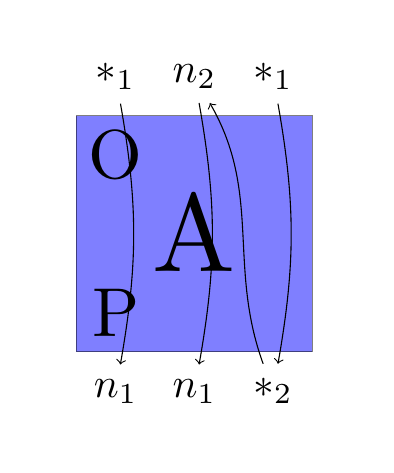
\begin{tikzpicture}
			 \node (inv) at (0,0) [minimum size=2pt] {};
			 \node (inv2) at (4,-5) [minimum size=2pt, scale=1.5] {};
			 
			 \draw [fill=blue, opacity=.5] (3.5,-4) rectangle (.5,-1);
			 \node (A) at (2,-2.5) [minimum size=2pt, scale=4] {A};
			 \node (P) at (1,-3.5) [minimum size=2pt, scale=2.5] {P};
			 \node (O) at (1,-1.5) [minimum size=2pt, scale=2.5] {O};
			 
			 \only<2>{
			 \node (st_12) at (1,-.5) [minimum size=2pt, scale=1.5] {$*_1$};
			 \node (ri_12) at (1,-4.5) [minimum size=2pt, scale=1.5] {$n_1$};
		
			 
			 \node (st_1) at (3,-.5) [minimum size=2pt, scale=1.5] {$*_1$};
			 \node (st_2) at (3,-4.5) [minimum size=2pt, scale=1.5] {$*_2$};
			 \node (ri_1) at (2,-.5) [minimum size=2pt, scale=1.5] {$n_2$};
			 \node (ri_2) at (2,-4.5) [minimum size=2pt, scale=1.5] {$n_1$};
			 
			  \draw[->] [out=280,in=80] (st_1) to (st_2);
			  \draw[->] [out=110,in=300] (st_2) to (ri_1);
			  \draw[->] [out=280,in=80] (ri_1) to (ri_2);
			  \draw[->] [out=280,in=80] (st_12) to (ri_12);
			}
			\end{tikzpicture}
		
	\end{column}
	\end{columns}
	\centering
	\onslide<2>
	Esempi di strategie:
	\begin{gather*}
	\sigma=\{\epsilon, *_1n_1\}\leftrightarrow f_\sigma(*_1)=n_1  \\
	\tau=\{\epsilon, \; *_1*_2, \; *_1*_2n_2n_1\}\leftrightarrow f_\tau(*_1)=*_2,\; f_\tau(n_2)=n_1
	\end{gather*}
	
\end{frame}

% ordine tra strategie
\begin{frame}
 
 Estendiamo la relazione $\approx$ alle strategie, ponendo:
 \pause
	\begin{itemize}
	\item $\underline{ \sigma \preccurlyeq_s \tau }$ se per ogni $sab \in \sigma$ e $s' \in \tau$ t.c. $sa\approx s'a'$, esiste $b'$ tale che $s'a'b' \in \tau$ e $sab\approx s'a'b'$
	\item $\underline{ \sigma \approx_s \tau \ } \; \text{sse} \; \sigma \preccurlyeq_s \tau \wedge \tau \preccurlyeq_s \sigma$
	\end{itemize}  
	\pause
In particolare, la definizione porta alcune conseguenze: 

	\begin{itemize}
		\item $\preccurlyeq_s$ è un preordine sulle strategie; di conseguenza $\approx_s$ è una relazione di equivalenza parziale
		\item Nel caso l'equivalenza $\approx$ del gioco sia l'identità, l'ordine tra strategie si può vedere come inclusione di insiemi o tra le funzioni parziali. Intuitivamente, $\sigma \preccurlyeq_s \tau$ se $\tau$ può fare più mosse di $\sigma$
	\end{itemize}
	
\end{frame}

% esempio di ordine
\begin{frame}
	\begin{columns}
	\begin{column}{0.45\textwidth}
	Gioco $A=( M_A , \lambda_A , P_A , \approx_A )$
		\begin{itemize}
		         	\item $M_{A}=\{*_1,*_2,n_1,n_2\}$
		           	\item $\lambda_{A}= \{ (*_1,OQ) ;$ $ (*_2,PQ) ; (n_1,PA) ; (n_2,OA) \}$
					\item $P_{A}= \{ 
					\epsilon ,$
					$ *_1 ,
					\; *_1n_1, $ 
					$ *_1*_2,
					\; *_1*_2n_2, 
					\; *_1*_2n_2n_1 \}$
					\item $\approx_{A} = id_{A}$        
		\end{itemize}
	\end{column}
	\begin{column}{0.4\textwidth}
		\begin{tikzpicture}
			 \node (inv) at (0,0) [minimum size=2pt] {};
			 \node (inv2) at (4,-5) [minimum size=2pt, scale=1.5] {};
			 
			 \draw [fill=blue, opacity=.5] (3.5,-4) rectangle (.5,-1);
			 \node (A) at (2,-2.5) [minimum size=2pt, scale=4] {A};
			 \node (P) at (1,-3.5) [minimum size=2pt, scale=2.5] {P};
			 \node (O) at (1,-1.5) [minimum size=2pt, scale=2.5] {O};
			 
			 \node (st_12) at (1,-.5) [minimum size=2pt, scale=1.5] {$*_1$};
			 \only<1-2>{\node (ri_12) at (1,-4.5) [minimum size=2pt, scale=1.5] {$n_1$};}
	 		 \only<3-4>{\node (st_22) at (1,-4.5) [minimum size=2pt, scale=1.5] {$*_2$};}
			 \node (st_1) at (3,-.5) [minimum size=2pt, scale=1.5] {$*_1$};
			 \node (st_2) at (3,-4.5) [minimum size=2pt, scale=1.5] {$*_2$};
			 \node (ri_1) at (2,-.5) [minimum size=2pt, scale=1.5] {$n_2$};
			 \node (ri_2) at (2,-4.5) [minimum size=2pt, scale=1.5] {$n_1$};
			 
			  \draw[->] [out=280,in=80] (st_1) to (st_2);
			  \draw[->] [out=110,in=300] (st_2) to (ri_1);
			  \draw[->] [out=280,in=80] (ri_1) to (ri_2);
			  \only<1-2>{\draw[->] [out=280,in=80] (st_12) to (ri_12);}
			  \only<3-4>{\draw[->] [out=280,in=80] (st_12) to (st_22);}
			\end{tikzpicture}
		
	\end{column}
	\end{columns}
	\centering
	\begin{gather*}
	\only<1-2>{\sigma=\{\epsilon, *_1n_1\}\leftrightarrow f_\sigma(*_1)=n_1  \\}
	\only<3-4>{\sigma=\{\only<4>{\textcolor{red}{\epsilon, \; *_1*_2}}\only<3>{\epsilon, \; *_1*_2}\}\leftrightarrow \only<4>{\textcolor{red}{f_\sigma(*_1)=*_2}}\only<3>{f_\sigma(*_1)=*_2}  \\}
	\tau=\{\only<4>{\textcolor{red}{\epsilon, \; *_1*_2}}\only<1-3>{\epsilon, \; *_1*_2}, \; *_1*_2n_2n_1\}\leftrightarrow 
	\only<4>{\textcolor{red}{f_\tau(*_1)=*_2}}\only<1-3>{f_\tau(*_1)=*_2},\; 
	f_\tau(n_2)=n_1
	\\
	\only<2>{\sigma \not\preccurlyeq_s \tau, \; \sigma \not\preccurlyeq_s \tau}
	\only<4>{\sigma \preccurlyeq_s \tau}
	\end{gather*}
\end{frame}

\subsection{operazioni tra giochi}

% prodotto tensore
\begin{frame}
	
	\frametitle{Il gioco $A \otimes B$}
	Dati due giochi $A$ e $B$ definiamo il gioco $A\otimes B$ come:
	\begin{itemize}
		\item<2-> $M_{A\otimes B}=M_A \coprod M_B$
		\item<3-> $\lambda_{A\otimes B}=\lambda_A \coprod \lambda_B$
		\item<4-> $P_{A\otimes B}$ sono tutte le partite $s$ tali che $s|_{M_A} \in P_A \wedge s|_{M_B} \in P_B$
		\begin{itemize}
			\item $s|_{M_A} \in P_A \wedge s|_{M_B} \in P_B$
			\item Per ogni domanda in $A$, la risposta deve essere in $A$; lo stesso con $B$
		\end{itemize}
		\item<5-> $s\approx_{A\otimes B} t \Leftrightarrow s|_A \approx_A t|_A \wedge s|_B \approx_B t|_B \wedge fst(s)=fst(t)$ 
	\end{itemize}
	
	\onslide<6-9>{
	\begin{block}{Proprietà}
		\begin{itemize}
			\item<7-> Il prodotto tensore è associativo
			\item<8-> Esiste un elemento neutro $I$, ossia il gioco vuoto
			\item<9-> \textcolor{red}{Solamente il giocatore $O$ può cambiare componente di gioco}
		\end{itemize}
		
	\end{block}
	}
	
\end{frame}

% esempio Prodotto Tensore
\begin{frame}[t]
\frametitle{Il gioco $A \otimes B$}

\pause
\begin{itemize}
 \item $A$ con $P_A=\{
 \only<3-7>{\textcolor{red}{\epsilon}} \only<1-2,8->{\epsilon},
 \;  \only<8-9>{\textcolor{red}{*_O}} \only<1-7,10->{*_O}, 
 \; \only<10->{\textcolor{red}{*_O\checkmark_P}} \only<1-9>{*_O\checkmark_P}, 
 \;*_O\times_P 
 \}$
 \item $B$ con $P_B=\{
 \only<3>{\textcolor{red}{\epsilon}} \only<1-2,4->{\epsilon},
 \;  \only<4-5>{\textcolor{red}{*_O}} \only<1-3,6->{*_O}, 
 \; *_O0_P,
 \; *_O1_P,
 \; \only<6->{\textcolor{red}{*_O2_P}} \only<1-5>{*_O2_P},
 \; *_O3_P,
 \; \dots \}$
\end{itemize}
\pause
\centering Descriviamo $A \otimes B$ tramite il tavolo di gioco

\begin{tikzpicture}
 
	 \node (inv) at (0,0) [minimum size=2pt] {};
 	 \node (inv2) at (11,-4) [minimum size=2pt] {};
	
	\draw [fill=blue, opacity=.5] (4.5,-4.3) rectangle (1,-.8);
	\draw [fill=red, opacity=.5] (9.5,-4.3) rectangle (6,-.8);
	 
	  \node (A) at (2.75,-2.55) [minimum size=2pt, scale=4] {A};
 	  \node (PA) at (1.5,-3.8) [minimum size=2pt, scale=3] {P};
  	  \node (OA) at (1.5,-1.3) [minimum size=2pt, scale=3] {O};
  
	  \node (B) at (7.75,-2.55) [minimum size=2pt, scale=4] {B};
 	  \node (PB) at (6.5,-3.8) [minimum size=2pt, scale=3] {P};
  	  \node (OB) at (6.5,-1.3) [minimum size=2pt, scale=3] {O};
  
	  \only<4-> {\node (st1) at (7.75,-.4) [minimum size=2pt, scale=2] {$*_O$};}
	  \only<5> {\node (false1) at (2.75,-4.7) [minimum size=2pt, scale=2] {?};}
	  \only<6-> {\node (ri1) at (7.75,-4.7) [minimum size=2pt, scale=2] {$2_P$};}
	  \only<7> {\node (false2) at (6.5,-.4) [minimum size=2pt, scale=2] {?};}
	  \only<8-> {\node (st2) at (2.75,-.4) [minimum size=2pt, scale=2] {$*_O$};}
	  \only<9> {\node (false3) at (6.5,-4.7) [minimum size=2pt, scale=2] {?};}
	  \only<10-> {\node (ri2) at (2.75,-4.7) [minimum size=2pt, scale=2] {$\checkmark_P$};}
	 
	 \only<5>{\draw[->] (st1) to (false1);}
	 
	 \only<6->{\draw[->] (st1) to (ri1);}
	 
	 \only<7>{\draw[->] (ri1) to (false2);}
	 
	 \only<8->{\draw[->] (ri1) to (st2);}
	 
	 \only<9>{\draw[->] (st2) to (false3);}
	 
	 \only<10->{\draw[->] (st2) to (ri2);}
	
	 
 
\end{tikzpicture}






	
\end{frame}


% gioco implicazione lineare
\begin{frame}
	
	\frametitle{Il gioco $A \limp B$}
	Dati due giochi $A$ e $B$ definiamo il gioco $A\limp B$ come:
	\begin{itemize}
		\item<2-> $M_{A\limp B}=M_A \coprod M_B$
		\item<3-> $\lambda^{QA}_{A\limp B}=\lambda^{QA}_A \coprod \lambda^{QA}_B$
		
		$\lambda^{OP}_{A\limp B}=\textcolor{red}{\overline{\lambda^{OP}_A}} \coprod \lambda^{OP}_B$
		\item<4-> $P_{A\otimes B}$ sono tutte le partite $s$ tali che:
		\begin{itemize}
			\item $s|_{M_A} \in P_A \wedge s|_{M_B} \in P_B$
			\item Per ogni domanda in $A$, la risposta deve essere in $A$; lo stesso con $B$
		\end{itemize}
		\item<5-> $s\approx_{A\otimes B} t \Leftrightarrow s|_A \approx_A t|_A \wedge s|_B \approx_B t|_B \wedge fst(s)=fst(t)$ 
	\end{itemize}
	\onslide<6>
	\begin{block}{Proprietà}
		
		\textcolor{red}{Solamente il giocatore $P$ può cambiare componente di gioco}
		
	
	\end{block}
	
\end{frame}

% esempio implicazione lineare
\begin{frame}[t]
\frametitle{Il gioco $A \limp B$}

\pause
\begin{itemize}
 \item $A$ con $P_A=\{
 \only<3-6>{\textcolor{red}{\epsilon}} \only<1-2,7->{\epsilon},
 \;  \only<7-8>{\textcolor{red}{*_O}} \only<1-6,9->{*_O}, 
 \; \only<9->{\textcolor{red}{*_O\checkmark_P}} \only<1-8>{*_O\checkmark_P}, 
 \;*_O\times_P 
 \}$
 \item $B$ con $P_B=\{
 \only<3-5>{\textcolor{red}{\epsilon}} \only<1-2,6->{\epsilon},
 \;  \only<6-10>{\textcolor{red}{*_O}} \only<1-5,11->{*_O}, 
 \; *_O0_P,
 \; *_O1_P,
 \; \only<11->{\textcolor{red}{*_O2_P}} \only<1-10>{*_O2_P},
 \; *_O3_P,
 \; \dots \}$
\end{itemize}
\pause
\centering Descriviamo $A \limp B$ tramite il tavolo di gioco

\begin{tikzpicture}
 
	 \node (inv) at (0,0) [minimum size=2pt] {};
 	 \node (inv2) at (11,-4) [minimum size=2pt] {};
	
	\draw [fill=blue, opacity=.5] (4.5,-4.3) rectangle (1,-.8);
	\draw [fill=red, opacity=.5] (9.5,-4.3) rectangle (6,-.8);
	 
	  \node (A) at (2.75,-2.55) [minimum size=2pt, scale=4] {A};
	  \only<3>{\node (Pfake) at (1.5,-3.8) [minimum size=2pt, scale=3] {\textcolor{red}{P}};}
  	  \only<3>{\node (Ofake) at (1.5,-1.3) [minimum size=2pt, scale=3] {\textcolor{red}{O}};}
 	  \only<4->{\node (PA) at (2.4,-1.3) [minimum size=2pt, scale=2.7] {P=O$_A$};}
  	  \only<4->{\node (OA) at (2.4,-3.8) [minimum size=2pt, scale=2.7] {O=P$_A$};}
  
	  \node (B) at (7.75,-2.55) [minimum size=2pt, scale=4] {B};
 	  \node (PB) at (6.5,-3.8) [minimum size=2pt, scale=3] {P};
  	  \node (OB) at (6.5,-1.3) [minimum size=2pt, scale=3] {O};
  
          \only<5> {\node (false1) at (2.75,-4.7) [minimum size=2pt, scale=2] {?};}
	  \only<6-> {\node (st1) at (7.75,-.4) [minimum size=2pt, scale=2] {$*_O$};}
	  \only<7-> {\node (st2) at (2.75,-.4) [minimum size=2pt, scale=2] {$*_O$};}
	  \only<8> {\node (false2) at (6.5,-.4) [minimum size=2pt, scale=2] {?};}
	  \only<9-> {\node (ri2) at (2.75,-4.7) [minimum size=2pt, scale=2] {$\checkmark_P$};}
	  \only<10> {\node (false3) at (1.5,-.4) [minimum size=2pt, scale=2] {?};}
	  \only<11-> {\node (ri1) at (7.75,-4.7) [minimum size=2pt, scale=2] {$2_P$};}
	  
	  
	 
	 \only<7->{\draw[->][out=220, in=340] (st1) to (st2);}
	 \only<8>{\draw[->] (st2) to (false2);}
	 \only<9->{\draw[->] (st2) to (ri2);}
	 \only<10>{\draw[->] (ri2) to (false3);}
	 \only<11->{\draw[->] (ri2) to (ri1);}
	 

	
	 
 
\end{tikzpicture}






	
\end{frame}

% gioco prodotto tensore infinito
\begin{frame}
	
	\frametitle{Il gioco $!A$}
	
	\begin{itemize}
		\item $M_{!A}=\omega \times M_A$
		\item $\lambda_{!A}(i,a)=\lambda_A(a)$
		\item $s$ è una partita di $P_{!A}$ se e solo se:
		\begin{itemize}
			\item $\forall i\in \omega , s|_i \in P_A$
			\item Se una domanda è nella componente $i$, la sua risposta deve essere nella componente $i$ (\emph{indexed bracketing condition})
		\end{itemize}

		\item $s\approx_{!A} t$ sse esiste $\pi:\omega \rightarrow \omega$ permutazione tale che $s|_i \approx_A t|_{\pi(i)} \wedge (\pi \circ fst)(s)=fst(t)$
	\end{itemize}
	
	\begin{block}{Proprietà}
		\begin{itemize}
			\item Solamente il giocatore $O$ può cambiare componente di gioco
		\end{itemize}
	\end{block}
	
	Nota: concettualmente il gioco $!A$ si comporta come se avessimo infinite copie di $A$ tensorizzate $A\otimes A\otimes A\otimes A\otimes \dots$ con la relazione $\approx_{!A}$
	
\end{frame}

% roulette russa
\begin{frame}
\frametitle{Il gioco $A\Rightarrow B$}

\only<2->{
	\[
	A \Rightarrow B \quad \equiv \quad !A \limp B
	\]
}

\only<1-10>{
\onslide<3->{
\begin{itemize}
 \item $Gun=A$ con $P_A=\{
 \only<3-5>{\textcolor{red}{\epsilon}} \only<1-2,6->{\epsilon},
 \;  \only<6,8>{\textcolor{red}{\underline{pull}}} \only<1-5,7,9->{\underline{pull}}, 
 \; \only<7>{\textcolor{red}{\underline{pull}\:click}} \only<1-6,8->{\underline{pull}\:click}, 
 \; \only<9->{\textcolor{red}{\underline{pull}\:bang}} \only<1-8>{\underline{pull}\:bang} 
 \}$
 \item $Life=B$ con $P_B=\{
 \only<3-4>{\textcolor{red}{\epsilon}} \only<1-2,5->{\epsilon},
 \;  \only<5-9>{\textcolor{red}{*_O}} \only<1-4,10->{*_O}, 
 \; *_O\checkmark_P,
 \; *_O1_P,
 \; \only<10->{\textcolor{red}{*_O2_P}} \only<1-9>{*_O2_P},
 \; *_O3_P,
 \; \dots \}$
 \item<4-> Strategia \textit{Roulette Russa}:
 
 $\only<6>{\textcolor{red}{f(*_O)=\underline{pull}_1}} \only<4-5,7->{f(*_O)=\underline{pull}_1}$, 
 $\quad \only<8>{\textcolor{red}{f(click_n)=\underline{pull}_{n+1}}} \only<4-7,9->{f(click_n)=\underline{pull}_{n+1}} \forall n$,  
 $\quad \only<10>{\textcolor{red}{f(bang_n)=n_P}} \only<4-9>{f(bang_n)=n_P}$
\end{itemize}
}
}


\only<11->{

\begin{itemize}
 \item $Gun=A$ con $P_A=\{
 \only<3-5>{\textcolor{red}{\epsilon}} \only<1-2,6->{\epsilon},
 \;  \only<6,8>{\textcolor{red}{\underline{pull}}} \only<1-5,7,9->{\underline{pull}}, 
 \; \only<7>{\textcolor{red}{\underline{pull}\:click}} \only<1-6,8->{\underline{pull}\:click}, 
 \; \only<9->{\textcolor{red}{\underline{pull}\:bang}} \only<1-8>{\underline{pull}\:bang} 
 \}$
 \item $Life=B$ con $P_B=\{
 \only<3-4>{\textcolor{red}{\epsilon}} \only<1-2,5->{\epsilon},
 \;  \only<5-9>{\textcolor{red}{*_O}} \only<1-4,10->{*_O}, 
 \; *_O\checkmark_P,
 \; *_O1_P,
 \; \only<10->{\textcolor{red}{*_O2_P}} \only<1-9>{*_O2_P},
 \; *_O3_P,
 \; \dots \}$
 \item Strategia \textit{Roulette Russa}:
 
 $\only<6>{\textcolor{red}{f(*_O)=\underline{pull}_2}} \only<4-5,7->{f(*_O)=\underline{pull}_2}$, 
 $\quad \only<8>{\textcolor{red}{f(click_{2n})=\underline{pull}_{2n+2}}} \only<4-7,9->{f(click_{2n})=\underline{pull}_{2n+2}} \forall n$,  
 $\quad \only<10->{\textcolor{red}{f(bang_{2n})=n_P}} \only<4-9>{f(bang_{2n})=n_P}$
\end{itemize}

}



\only<2-10>{ 
	\begin{tikzpicture}
	 \node (inv) at (0,0) [minimum size=2pt] {};
	 \node (inv2) at (11,-4) [minimum size=2pt] {};
	 \foreach \x in {0,3,6} { 
	  \draw [fill=blue, opacity=.5] (\x+2,-3) rectangle (\x,-1);
	 % \node (A) at (\x+1,-2) [minimum size=2pt, scale=2] {A};
	  \node (P) at (\x+0.3,-1.3) [minimum size=2pt, scale=1.5] {P};
 	  \node (O) at (\x+0.3,-2.7) [minimum size=2pt, scale=1.5] {O};
	  }
	  \node (A) at (7,-2) [minimum size=2pt, scale=2] {A$_1$};
	  \node (A) at (4,-2) [minimum size=2pt, scale=2] {A$_2$};
	  \node (A) at (1,-2) [minimum size=2pt, scale=2] {A$_3$};
	 \draw [fill=red, opacity=.5] (11,-3) rectangle (9,-1);
	 \node (B) at (10,-2) [minimum size=2pt, scale=2] {B};
	 \node (P) at (9.3,-2.7) [minimum size=2pt, scale=1.5] {P};
 	 \node (O) at (9.3,-1.3) [minimum size=2pt, scale=1.5] {O};
	 
	 \only<5->{\node (st1) at (10,-0.5) [minimum size=2pt, scale=1.5] {$*_O$};}
 	 \only<6->{\node (st2) at (7,-0.5) [minimum size=2pt, scale=1.5] {$\underline{pull}_1$};}
	 \only<7->{\node (ri2) at (7,-3.5) [minimum size=2pt, scale=1.5] {$click_1$};}
 	 \only<8->{\node (st3) at (4,-0.5) [minimum size=2pt, scale=1.5] {$\underline{pull}_2$};}
	 \only<9->{\node (ri3) at (4,-3.5) [minimum size=2pt, scale=1.5] {$bang_2$};}
 	 \only<10->{\node (ri1) at (10,-3.5) [minimum size=2pt, scale=1.5] {$2_P$};}
 	 
	  \only<6->{\draw[->] [out=250,in=280] (st1) to (st2);}
	  \only<7->{\draw[->] [out=250,in=30] (st2) to (ri2);}
	  \only<8->{\draw[->] [out=80,in=280] (ri2) to (st3);}
	  \only<9->{\draw[->] [out=250,in=110] (st3) to (ri3);}
	  \only<10->{\draw[->] [out=30,in=150] (ri3) to (ri1);}
	  \end{tikzpicture}

	}

	
\only<11->{ 
	\begin{tikzpicture}
	 \node (inv) at (0,0) [minimum size=2pt] {};
	 \node (inv2) at (11,-4) [minimum size=2pt] {};
	 \foreach \x in {0,3,6} { 
	  \draw [fill=blue, opacity=.5] (\x+2,-3) rectangle (\x,-1);
	 % \node (A) at (\x+1,-2) [minimum size=2pt, scale=2] {A};
	  \node (P) at (\x+0.3,-1.3) [minimum size=2pt, scale=1.5] {P};
 	  \node (O) at (\x+0.3,-2.7) [minimum size=2pt, scale=1.5] {O};
	  }
	  \node (A) at (7,-2) [minimum size=2pt, scale=2] {A$_2$};
	  \node (A) at (4,-2) [minimum size=2pt, scale=2] {A$_4$};
	  \node (A) at (1,-2) [minimum size=2pt, scale=2] {A$_6$};
	 \draw [fill=red, opacity=.5] (11,-3) rectangle (9,-1);
	 \node (B) at (10,-2) [minimum size=2pt, scale=2] {B};
	 \node (P) at (9.3,-2.7) [minimum size=2pt, scale=1.5] {P};
 	 \node (O) at (9.3,-1.3) [minimum size=2pt, scale=1.5] {O};
	 
	 \only<5->{\node (st1) at (10,-0.5) [minimum size=2pt, scale=1.5] {$*_O$};}
 	 \only<6->{\node (st2) at (7,-0.5) [minimum size=2pt, scale=1.5] {$\underline{pull}_2$};}
	 \only<7->{\node (ri2) at (7,-3.5) [minimum size=2pt, scale=1.5] {$click_2$};}
 	 \only<8->{\node (st3) at (4,-0.5) [minimum size=2pt, scale=1.5] {$\underline{pull}_4$};}
	 \only<9->{\node (ri3) at (4,-3.5) [minimum size=2pt, scale=1.5] {$bang_4$};}
 	 \only<10->{\node (ri1) at (10,-3.5) [minimum size=2pt, scale=1.5] {$2_P$};}
 	 
	  \only<6->{\draw[->] [out=250,in=280] (st1) to (st2);}
	  \only<7->{\draw[->] [out=250,in=30] (st2) to (ri2);}
	  \only<8->{\draw[->] [out=80,in=280] (ri2) to (st3);}
	  \only<9->{\draw[->] [out=250,in=110] (st3) to (ri3);}
	  \only<10->{\draw[->] [out=30,in=150] (ri3) to (ri1);}
	  \end{tikzpicture}

	}
	
\end{frame}


\subsection{strategie importanti}

% strategia composizione con esempio
\begin{frame}

	\frametitle{La strategia $\sigma ; \tau$}
Date $\sigma$ strategia di $A\limp B$ e $\tau$ di $B\limp C$, allora

\begin{itemize}
 \item<2-> $\sigma ; \tau =\{s|_{A,C} : s \in (M_A \coprod M_B \coprod M_C)^*, \; s|_{A,B} \in \sigma, \; s|_{B,C} \in \tau \}$
 \item<3-> $\sigma ; \tau$ è una strategia di $A\limp C$
\end{itemize}

\onslide<4->{Si può dare una costruzione di $\sigma ; \tau$ algoritmica:}

\only<-13>{
\begin{tikzpicture}
			 \node (inv) at (0,0) [minimum size=2pt] {};
			 \node (inv2) at (11,-5) [minimum size=2pt, scale=1.5] {};
			
			\only<5->{
			 \draw [fill=blue, opacity=.5] (1.9,-3.5) rectangle (-.1,-1.5);
			 \draw [fill=red, opacity=.5] (4.9,-3.5) rectangle (2.9,-1.5);
			 \draw [fill=red, opacity=.5] (7.4,-3.5) rectangle (5.4,-1.5);
			 \draw [fill=green, opacity=.5] (10.4,-3.5) rectangle (8.4,-1.5);
			 			 
			 \node (A) at (.9,-2.5) [minimum size=2pt, scale=2] {A};
			 \node (B) at (3.9,-2.5) [minimum size=2pt, scale=2] {B};
			 \node (B) at (6.4,-2.5) [minimum size=2pt, scale=2] {B};
			 \node (C) at (9.4,-2.5) [minimum size=2pt, scale=2] {C};
			 
			 \node (P) at (.2,-1.8) [minimum size=2pt, scale=1.5] {P};
			 \node (P) at (3.2,-3.2) [minimum size=2pt, scale=1.5] {P};
			 \node (P) at (5.7,-1.8) [minimum size=2pt, scale=1.5] {P};
			 \node (P) at (8.7,-3.2) [minimum size=2pt, scale=1.5] {P};
			 
			 \node (O) at (.2,-3.2) [minimum size=2pt, scale=1.5] {O};
			 \node (O) at (3.2,-1.8) [minimum size=2pt, scale=1.5] {O};
			 \node (O) at (5.7,-3.2) [minimum size=2pt, scale=1.5] {O};
			 \node (O) at (8.7,-1.8) [minimum size=2pt, scale=1.5] {O};
			 
			 %\node (O) at (1,-1.5) [minimum size=2pt, scale=2.5] {O};
			 
			 \node (sigma) at (2.3,-.3) [minimum size=2pt, scale=2] {\only<8,10,12>{\textcolor{red}{$\sigma$}} \only<1-7,9,11,13>{$\sigma$}};
			 \node (tau) at (7.9,-.3) [minimum size=2pt, scale=2] {\only<7,9,13>{\textcolor{red}{$\tau$}} \only<1-6,8,10-12>{$\tau$}};
			\draw[dashed] (5.15, -4.5) -- (5.15, -.5);
			}
			
			
			\only<6->{ \node (st_1) at (9.4,-1) [minimum size=2pt, scale=1.5] {$*_1$};}
			\only<7->{\node (st_2) at (6.9,-1) [minimum size=2pt, scale=1.5] {$*_2$};}
			 \only<7->{\node (st_2b) at (4.4,-1) [minimum size=2pt, scale=1.5] {$*_2$};}
			\only<8->{  \node (ri_2) at (6.9,-4) [minimum size=2pt, scale=1.5] {$n_2$};}
			 \only<8->{ \node (ri_2b) at (4.4,-4) [minimum size=2pt, scale=1.5] {$n_2$};}
			 \only<9->{\node (st_3) at (5.9,-1) [minimum size=2pt, scale=1.5] {$*_3$};}
			\only<9->{ \node (st_3b) at (3.4,-1) [minimum size=2pt, scale=1.5] {$*_3$};}
			 \only<10->{\node (st_4) at (.9,-1) [minimum size=2pt, scale=1.5] {$*_4$};}
			 \only<11->{\node (ri_4) at (.9,-4) [minimum size=2pt, scale=1.5] {$n_4$};}
			 \only<12->{\node (ri_3b) at (3.4,-4) [minimum size=2pt, scale=1.5] {$n_3$};}
			\only<12->{ \node (ri_3) at (5.9,-4) [minimum size=2pt, scale=1.5] {$n_3$};}
			\only<13->{ \node (ri_1) at (9.4,-4) [minimum size=2pt, scale=1.5] {$n_1$};}
			 
			 %\node (ri_2) at (2,-4.5) [minimum size=2pt, scale=1.5] {$n_1$};
			 
			 \only<7->{ \draw[->] (st_1) to (st_2);}
			  \only<8->{\draw[dashed,->] (st_2) to (ri_2);}
			  \only<8->{\draw[->] (st_2b) to (ri_2b);}
			  \only<9->{\draw[->] (ri_2) to (st_3);}
			 \only<9->{ \draw[dashed,->] (ri_2b) to (st_3b);}
			\only<10->{  \draw[->] (st_3b) to (st_4);}
			 \only<11->{ \draw[->] (st_4) to (ri_4);}
			 \only<12->{ \draw[dashed,->] (st_3) to (ri_3);}
			 \only<12->{ \draw[->] (ri_4) to (ri_3b);}
			 \only<13->{ \draw[->] [in=150, out=30] (ri_3) to (ri_1);}
			  
			  %\draw[->] [out=180,in=300] (st_2) to (ri_1);
			  %\draw[->] [out=280,in=0] (ri_1) to (ri_2);
			
			\end{tikzpicture}
}

\only<14->{
\begin{tikzpicture}
			 \node (inv) at (0,0) [minimum size=2pt] {};
			 \node (inv2) at (11,-5) [minimum size=2pt, scale=1.5] {};
			
			\only<5->{
			 \draw [fill=blue, opacity=.5] (1.9,-3.5) rectangle (-.1,-1.5);
			 \draw [fill=red, opacity=.1] (4.9,-3.5) rectangle (2.9,-1.5);
			 \draw [fill=red, opacity=.1] (7.4,-3.5) rectangle (5.4,-1.5);
			 \draw [fill=green, opacity=.5] (10.4,-3.5) rectangle (8.4,-1.5);
			 			 
			 \node (A) at (.9,-2.5) [minimum size=2pt, scale=2] {A};
			 \node (B) at (3.9,-2.5) [opacity=.1, minimum size=2pt, scale=2] {B};
			 \node (B) at (6.4,-2.5) [opacity=.1, minimum size=2pt, scale=2] {B};
			 \node (C) at (9.4,-2.5) [minimum size=2pt, scale=2] {C};
			 
			 \node (P) at (.2,-1.8) [minimum size=2pt, scale=1.5] {P};
			 \node (P) at (3.2,-3.2) [opacity=.1, minimum size=2pt, scale=1.5] {P};
			 \node (P) at (5.7,-1.8) [opacity=.1, minimum size=2pt, scale=1.5] {P};
			 \node (P) at (8.7,-3.2) [minimum size=2pt, scale=1.5] {P};
			 
			 \node (O) at (.2,-3.2) [minimum size=2pt, scale=1.5] {O};
			 \node (O) at (3.2,-1.8) [opacity=.1, minimum size=2pt, scale=1.5] {O};
			 \node (O) at (5.7,-3.2) [opacity=.1, minimum size=2pt, scale=1.5] {O};
			 \node (O) at (8.7,-1.8) [minimum size=2pt, scale=1.5] {O};
			 
			 %\node (O) at (1,-1.5) [minimum size=2pt, scale=2.5] {O};
			 
			 \node (sigma) at (2.3,-.3) [minimum size=2pt, scale=2] {\only<8,10,12>{\textcolor{red}{$\sigma$}} \only<1-7,9,11,13>{$\sigma$}};
			 \node (tau) at (7.9,-.3) [minimum size=2pt, scale=2] {\only<7,9,13>{\textcolor{red}{$\tau$}} \only<1-6,8,10-12>{$\tau$}};
			\draw[opacity=.1, dashed] (5.15, -4.5) -- (5.15, -.5);
			}
			
			\node (st) at (5.15, -.3)[minimum size=2pt, scale=2] {$\sigma ; \tau$};
			
			
			\only<6->{ \node (st_1) at (9.4,-1) [minimum size=2pt, scale=1.5] {$*_1$};}
			\only<7->{\node (st_2) at (6.9,-1) [opacity=.1, minimum size=2pt, scale=1.5] {$*_2$};}
			 \only<7->{\node (st_2b) at (4.4,-1) [opacity=.1, minimum size=2pt, scale=1.5] {$*_2$};}
			\only<8->{  \node (ri_2) at (6.9,-4) [opacity=.1, minimum size=2pt, scale=1.5] {$n_2$};}
			 \only<8->{ \node (ri_2b) at (4.4,-4) [opacity=.1, minimum size=2pt, scale=1.5] {$n_2$};}
			 \only<9->{\node (st_3) at (5.9,-1) [opacity=.1, minimum size=2pt, scale=1.5] {$*_3$};}
			\only<9->{ \node (st_3b) at (3.4,-1) [opacity=.1, minimum size=2pt, scale=1.5] {$*_3$};}
			 \only<10->{\node (st_4) at (.9,-1) [minimum size=2pt, scale=1.5] {$*_4$};}
			 \only<11->{\node (ri_4) at (.9,-4) [minimum size=2pt, scale=1.5] {$n_4$};}
			 \only<12->{\node (ri_3b) at (3.4,-4) [opacity=.1, minimum size=2pt, scale=1.5] {$n_3$};}
			\only<12->{ \node (ri_3) at (5.9,-4) [opacity=.1, minimum size=2pt, scale=1.5] {$n_3$};}
			\only<13->{ \node (ri_1) at (9.4,-4) [minimum size=2pt, scale=1.5] {$n_1$};}
			 
			 %\node (ri_2) at (2,-4.5) [minimum size=2pt, scale=1.5] {$n_1$};
			 
			 \only<7->{ \draw[opacity=.1, ->] (st_1) to (st_2);}
			  \only<8->{\draw[opacity=.1, dashed,->] (st_2) to (ri_2);}
			  \only<8->{\draw[opacity=.1, ->] (st_2b) to (ri_2b);}
			  \only<9->{\draw[opacity=.1, ->] (ri_2) to (st_3);}
			 \only<9->{ \draw[opacity=.1, dashed,->] (ri_2b) to (st_3b);}
			\only<10->{  \draw[opacity=.1, ->] (st_3b) to (st_4);}
			 \only<11->{ \draw[->] (st_4) to (ri_4);}
			 \only<12->{ \draw[opacity=.1, dashed,->] (st_3) to (ri_3);}
			 \only<12->{ \draw[opacity=.1, ->] (ri_4) to (ri_3b);}
			 \only<13->{ \draw[opacity=.1, ->] [in=150, out=30] (ri_3) to (ri_1);}
			 
			 \draw[->] [in=360, out=200] (st_1) to (st_4);
			 \draw[->] [in=160, out=20] (ri_4) to (ri_1);
			  
			  %\draw[->] [out=180,in=300] (st_2) to (ri_1);
			  %\draw[->] [out=280,in=0] (ri_1) to (ri_2);
			
			\end{tikzpicture}
	}		
			
\end{frame}

% strategia copycat con esempio
\begin{frame}

	\frametitle{La strategia \emph{copycat} su $A\limp A$}
Dato un gioco $A$, è sempre possibile costruire la strategia \emph{copycat} su $A\limp A$:

\begin{itemize}
 \item +
\end{itemize}


\end{frame}



\subsection{esistenza del modello}

% categoria dei giochi
\begin{frame}
 	
 	\frametitle{La categoria dei giochi $\mathcal{G}$}
 	
 	Definiamo $\mathcal{G}$ la categoria tale che:
 	\begin{itemize}
 		\item $\mathcal{G}_0$ sono i giochi
 		\item dati due giochi $A$ e $B$, i morfismi $A\rightarrow B$ sono $\{ \sigma \text{ strategia di } A\limp B \;|\; \sigma \approx_s \sigma \} / \approx_s$
 		\item Date $[\sigma] : A\rightarrow B$ e $[\tau] : B \rightarrow C$, $[\tau] \circ [\sigma] = [\sigma ; \tau]$
		\item Il morfismo identico è dato dalla strategia $id_A$
 	\end{itemize}
 	
 	In particolare abbiamo che $\mathcal{G}$:
 	\begin{itemize}
 		\item è dotata di un oggetto finale ($1$)
 		\item è una categoria monoidale 
 		
 		($\otimes$ è un bifuntore associativo con elemento neutro)
 		\item è una categoria autonoma 
 		
 		(per ogni gioco $A$ esiste il suo gioco duale $1 \limp A$)
 		\item NON è una categoria cartesiana chiusa (mancano i prodotti)
 	\end{itemize}
 	
 \end{frame}

 % gioco unione
\begin{frame}
	
	\frametitle{Il gioco $A \& B$}
	
	\begin{itemize}
		\item $M_{A\& B}=M_A \coprod M_B$
		\item $\lambda_{A\& B}=\lambda_A \coprod \lambda_B$
		\item $P_{A\& B}=P_A \coprod P_B$
		\item $\approx_{A\& B} \; = \; \approx_A \coprod \approx_B$ 
	\end{itemize}
	
	\begin{block}{Proprietà}
		\begin{itemize}
			\item Una partita di $A\& B$ è giocata su una sola delle due componenti
			\item Ogni strategia di $A\& B$ è unione di una strategia di $A$ e di una strategia di $B$ (anche vuota)
		\end{itemize}
		
	\end{block}
	
\end{frame}

% dag e der
\begin{frame}[t]
Definire dag e der
\end{frame}


% categoria di co-Kleisli
\begin{frame}

Definiamo $K_!(\mathcal{G})$ la categoria di \emph{co-Kleisli} di $\mathcal{G}$ rispetto a $!$

In particolare:
	
	\begin{itemize}
		\item $K_!(\mathcal{G})_0 = \mathcal{G}_0$
		\item Dati due giochi $A,B$, $Mor_{K_!(\mathcal{G})}(A,B) = Mor_{\mathcal{G}}(!A,B)$
		\item Date due strategie $\sigma$ e $\tau$, $\tau \circ \sigma = \sigma \fatsemi \tau := \sigma ^\dag ; \tau$
		\item Dato un gioco $A$, il morfismo identico è $der_A$
	\end{itemize}

	In particolare $K_!(\mathcal{G})$ è una \emph{categoria cartesiana chiusa}, cioè:
	\begin{itemize}
		\item Dati due oggetti esiste il \emph{prodotto} ($A\& B$)
		\item Esiste un oggetto \emph{finale} ($1$)
		\item Dati due oggetti, esiste l'oggetto esponente 
		
		(``$\Rightarrow$'' è tale che $Mor_{K_!(\mathcal{G})}(A\& B,C) \cong Mor_{K_!(\mathcal{G})}(A,B\Rightarrow C)$)
	\end{itemize}

\end{frame}

% ppo e ccc razionale
\begin{frame}
	
	\frametitle{order enrichement}
	
	Definiamo un \emph{pointed poset (ppo)} come un poset con un minimo (generalmente indicato con $\perp$)
	
	Definiamo una categoria cartesiana chiusa $C$ \emph{pointed poset enriched} se:
	\begin{itemize}
		\item Dati due oggetti $A,B$, $(Mor(A,B),\sqsubseteq _{A,B},\perp _{A,B})$ è un pointed poset
		\item Composizione, prodotto e currying sono monotoni
		\item Per ogni $f: A\rightarrow B$, per ogni gioco $C$, $\perp_{B,C} \circ f = \perp _{A,B}$
	\end{itemize}
	
	Definiamo una categoria cartesiana chiusa $C$ \emph{razionale} se:
	\begin{itemize}
		\item è ppo-enriched
		\item per ogni $f: A\times B \rightarrow B$ si ha:
		\begin{itemize}
			\item La catena $(f^{(k)} | k\in \omega)$ definita da $f^{(0)}=\perp _{A,B}$ e $f^{k+1} = f \circ <id_A , f^{(k)}>$ ammette \emph{least upper bound} $f^{\triangledown}$
			\item Dati $g:C\rightarrow A$ e $h:B\rightarrow D$, $g\circ f^\triangledown \circ h = \bigsqcup_{k\in \omega} g \circ f^{(k)} \circ h$
		\end{itemize}

	\end{itemize}
	
\end{frame}

% I giochi sono un modello di PCF
\begin{frame}
	
	Dato $A$ gioco, date $[\sigma],[\tau]$ classi di strategie di $A$, definiamo
	\[[\sigma] \sqsubseteq [\tau] \Leftrightarrow \sigma \preccurlyeq_s \tau\]
% 	NOTA: con l'equinvalenza banale, non c'è bisogno di parlare di classi
	\begin{block}{Teorema}
		$K_! (\mathcal{G})$ con l'ordine $\sqsubseteq$ è razionale
	\end{block}
	
	\begin{block}{Teorema}
		Sia $C$ una categoria cartesiana chiusa razionale. Si ha che:
		\begin{itemize}
			\item Fissata la denotazione dei tipi base di PCF in $C$ (ogni tipo viene denotato con un oggetto)
			\item Fissata la denotazione delle costanti di PCF in $C$ (ogni termine di tipo $\tau$ viene denotato con un morfismo di $1\rightarrow \llbracket \tau \rrbracket$)
		\end{itemize}
		allora la denotazione può essere estesa a tutti i termini di PCF
		
	\end{block}
	
\end{frame}


\end{document}
